\chapter{Typesetting Examples}
\label{chapter:typesetting}

\emph{This chapter shows how to use the math, unit and figure tools set up in the preamble of \texttt{report.tex}. Look at the source of this file to see the commands, and remove the chapter before submitting.}

\section{Equations}
\label{sec:equations}

A numbered equation gets a \texttt{\textbackslash label}, so it can be referenced with \texttt{\textbackslash cref}, which adds the word ``equation'' automatically. The scalar Helmholtz equation for a monochromatic field $U(\vect{r})$ with wavenumber $k = 2\pi/\lambda$ is
\begin{equation}
    \label{eq:helmholtz}
    \nabla^2 U(\vect{r}) + k^2 U(\vect{r}) = 0 .
\end{equation}
Multi-line derivations use \texttt{align}. Use \texttt{\textbackslash notag} for lines that should not get a number:
\begin{align}
    \vect{E}(\vect{r}, t) &= \Re\left\{ \vect{E}_0 \, \e^{\iu (\vect{k} \cdot \vect{r} - \omega t)} \right\} \notag \\
                          &= \vect{E}_0 \cos(\vect{k} \cdot \vect{r} - \omega t),
    \label{eq:planewave}
\end{align}
where $\vect{k} = k \uvec{z}$ for a wave propagating along $z$. \Cref{eq:helmholtz,eq:planewave} show that \texttt{\textbackslash cref} also handles several labels at once.

\subsection{Derivatives}

The \texttt{derivative} package typesets derivatives consistently, with an upright differential $\odif{x}$:
\begin{equation}
    \odv{\phi}{t}, \qquad
    \pdv{U}{x}, \qquad
    \pdv[order=2]{U}{z}, \qquad
    \pdv{U}{x,y}, \qquad
    \int_{-\infty}^{\infty} \abs{U(x)}^2 \odif{x}.
\end{equation}
The wave equation becomes
\begin{equation}
    \nabla^2 \vect{E} - \frac{n^2}{c^2} \pdv[order=2]{\vect{E}}{t} = \vect{0}.
\end{equation}

\subsection{Notation macros}

Define notation once in the preamble and use the macro everywhere. To change how all vectors look (for example with arrows instead of bold), only the definition of \texttt{\textbackslash vect} needs editing. Some examples for Fourier optics:
\begin{align}
    \FT\{\rect(x)\}      &= \sinc(f_x), \\
    I(x, y)              &= \avg*{\abs*{U(x, y)}^2} = U \conj{U}, \\
    \phi(x, y)           &= \arg\{U(x, y)\} = \arctan\frac{\Im\{U\}}{\Re\{U\}}.
\end{align}
The starred versions \texttt{\textbackslash abs*} and \texttt{\textbackslash avg*} scale the delimiters to their content.

\section{Units and numbers}
\label{sec:units}

Always write quantities with \texttt{siunitx}. This gives the correct spacing, upright units and a consistent style:
\begin{itemize}
    \item a HeNe laser at \qty{632.8}{nm} with a coherence length of \qty{0.2}{m};
    \item a measured step height of \qty{125.4(12)}{nm}, where the uncertainty is written in brackets;
    \item a scan range of \qtyrange{-50}{50}{\micro m} with \qtylist{1;2;5}{\micro m} steps;
    \item a scan velocity of \qty{2.5}{mm/s}, a large number \num{1.2e6}, and angles such as \ang{45} or \qty{12}{\degree} (the shortcut \texttt{\textbackslash deg} gives a bare degree sign in running text, like 12\deg).
\end{itemize}

\section{Tables}
\label{sec:tables}

Use \texttt{booktabs} rules and the siunitx \texttt{S} column to align numbers on the decimal point (see \cref{tab:wavelengths}).

\begin{table}[htb]
    \centering
    \caption{Common laser wavelengths in optical metrology.}
    \label{tab:wavelengths}
    \begin{tabular}{l S[table-format=4.1] S[table-format=1.2e1]}
        \toprule
        Source    & {Wavelength (\unit{nm})} & {Coherence length (\unit{m})} \\
        \midrule
        HeNe      & 632.8  & 2.00e-1 \\
        Nd:YAG    & 1064.0 & 1.00e0  \\
        SLD       & 840.0  & 2.50e-5 \\
        \bottomrule
    \end{tabular}
\end{table}

\section{Figures and plots}
\label{sec:figures}

Plots can be drawn directly with \texttt{pgfplots}, so they use the font of the thesis. \Cref{fig:interference} shows two-beam interference, $I = I_1 + I_2 + 2\sqrt{I_1 I_2}\cos\Delta\phi$, and single-slit diffraction. For measured data, use \texttt{\textbackslash addplot table \{data.csv\};}. Figures exported from Python or MATLAB as PDF go in \texttt{\textbackslash includegraphics}.

\begin{figure}[htb]
    \centering
    \begin{subfigure}[b]{0.48\textwidth}
        \centering
        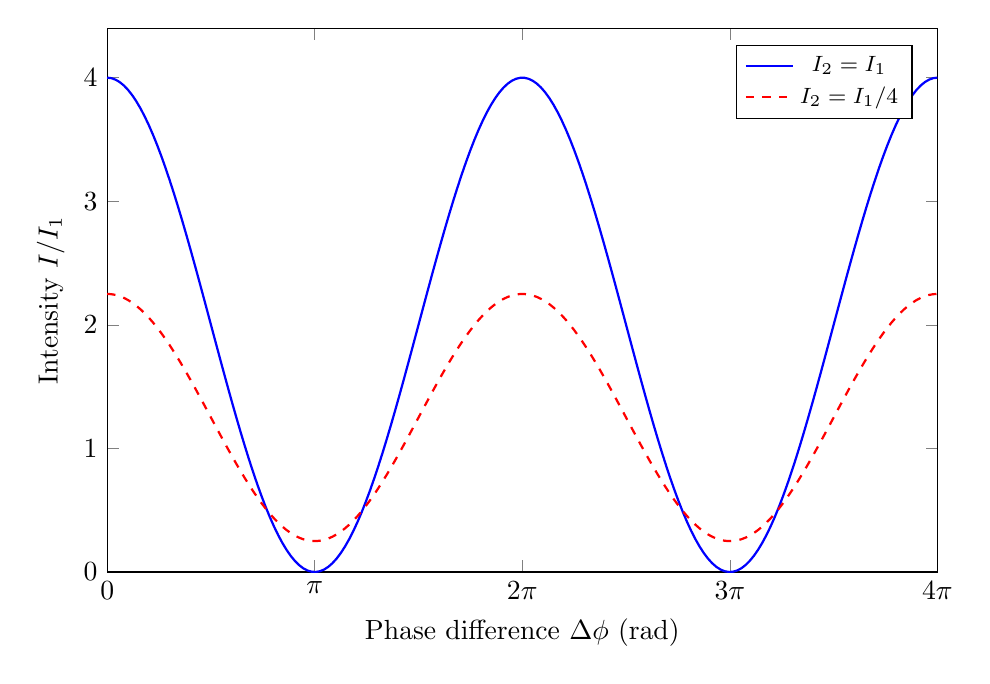
\begin{tikzpicture}
            \begin{axis}[
                width=\linewidth, height=0.7\linewidth,
                xlabel={Phase difference $\Delta\phi$ (\unit{rad})},
                ylabel={Intensity $I / I_1$},
                xmin=0, xmax=4*pi, ymin=0,
                xtick={0, pi, 2*pi, 3*pi, 4*pi},
                xticklabels={$0$, $\pi$, $2\pi$, $3\pi$, $4\pi$},
                legend pos=north east, legend style={font=\footnotesize},
            ]
                \addplot[domain=0:4*pi, samples=200, thick, blue] {2 + 2*cos(deg(x))};
                \addlegendentry{$I_2 = I_1$}
                \addplot[domain=0:4*pi, samples=200, thick, red, dashed] {1.25 + 2*sqrt(0.25)*cos(deg(x))};
                \addlegendentry{$I_2 = I_1/4$}
            \end{axis}
        \end{tikzpicture}
        \caption{Two-beam interference.}
        \label{fig:interference-twobeam}
    \end{subfigure}
    \hfill
    \begin{subfigure}[b]{0.48\textwidth}
        \centering
        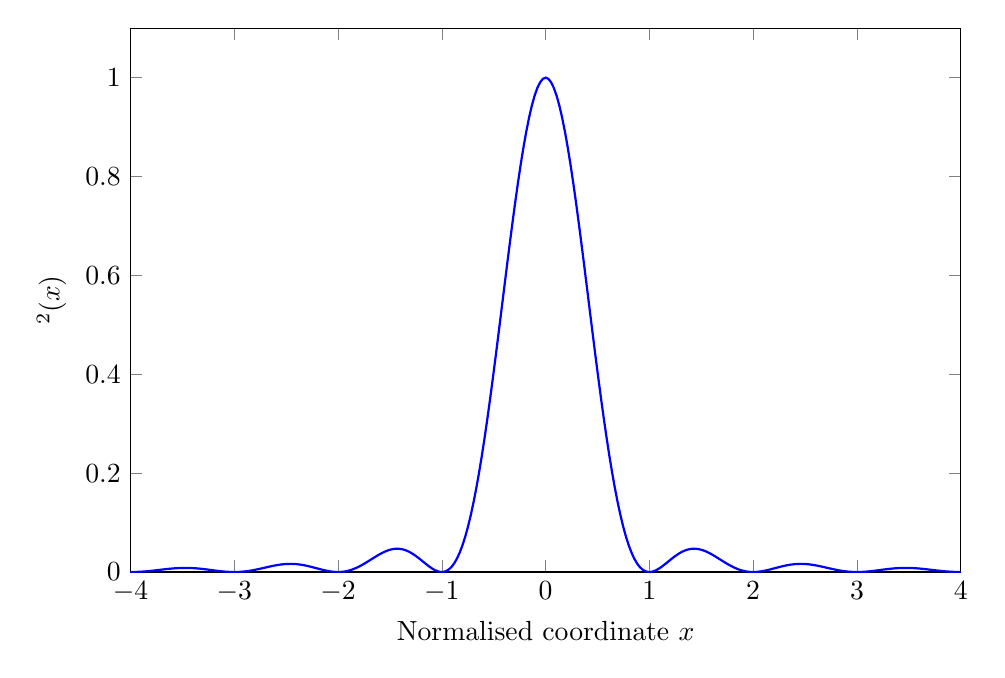
\begin{tikzpicture}
            \begin{axis}[
                width=\linewidth, height=0.7\linewidth,
                xlabel={Normalised coordinate $x$},
                ylabel={$\sinc^2(x)$},
                xmin=-4, xmax=4, ymin=0,
            ]
                \addplot[domain=-4:4, samples=301, thick, blue]
                    {x==0 ? 1 : (sin(deg(pi*x))/(pi*x))^2};
            \end{axis}
        \end{tikzpicture}
        \caption{Single-slit diffraction.}
        \label{fig:interference-slit}
    \end{subfigure}
    \caption{Examples of plots made with \texttt{pgfplots}.}
    \label{fig:interference}
\end{figure}

\section{Cross-references, citations and notes}
\label{sec:crossref}

\begin{itemize}
    \item \texttt{\textbackslash cref\{fig:interference-twobeam\}} gives ``\cref{fig:interference-twobeam}''. At the start of a sentence use \texttt{\textbackslash Cref}: ``\Cref{sec:units}''.
    \item Citations use the IEEE style: \texttt{\textbackslash cite\{example-article\}} gives \cite{example-article}.
    \item Margin notes for drafting are made with \texttt{\textbackslash todo\{...\}}.\todo{Example note: remove this chapter before submission.} To hide all notes in the final version, load \texttt{todonotes} with the \texttt{disable} option.
\end{itemize}
